\subsubsection{Ping Test}
\subsubsection{Frage 1}
\paragraph{Frage}
Wie kann von einem User PC auf einen Admin PC zugegriffen werden?
\paragraph{Antwort}
\textbf{Lösung 1:} Da VLAN die Ports auf Layer 2 separiert, könnte man ein Layer 3 Gerät, wie ein Router einfügen und den Default Gateway konfigurieren. Damit sollten Systeme auf beiden VLANs in der Lage sein, miteinander zu kommunizieren.
\\
\textbf{Lösung 2:} Eine weitere Lösung wäre die Ports an den Endsystem auf trunk mode zu ändern und sie für vlan 10 und 20 zu konfigurieren und den native trunk auf 10 oder 20 zu ändern.
\paragraph{Test für Lösung 1}
\begin{figure}[!htb]
    \centering
    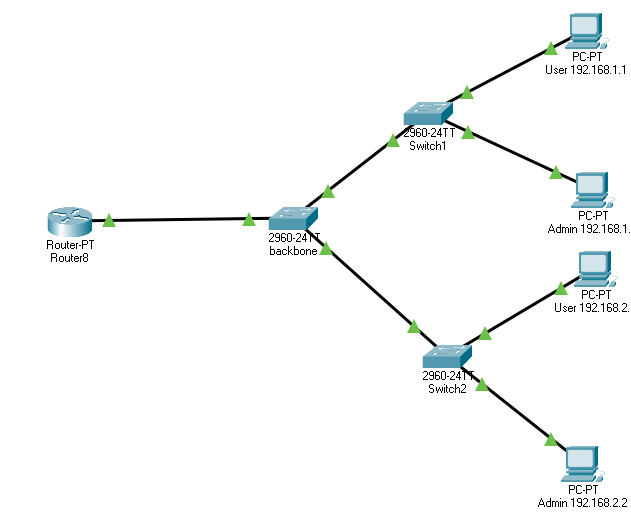
\includegraphics[width=\textwidth,height=.55\textwidth,keepaspectratio]{./img/test1/aufbau.png}
    \caption{Netz}
\end{figure}
\begin{figure}[!htb]
    \centering
    \begin{subfigure}{.45\textwidth}
        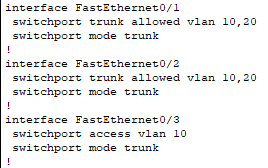
\includegraphics[width=\textwidth,height=\textwidth,keepaspectratio]{./img/test1/backbone.png}
        \caption{Backbone}
    \end{subfigure}
    \begin{subfigure}{.45\textwidth}
        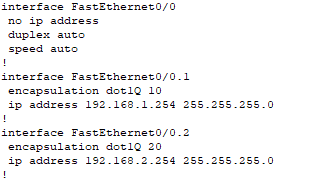
\includegraphics[width=\textwidth,height=\textwidth,keepaspectratio]{./img/test1/router.png}
        \caption{Router}
    \end{subfigure}
    ~
    \begin{subfigure}{.45\textwidth}
        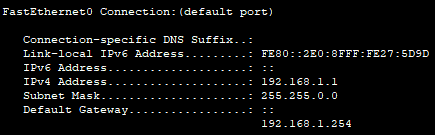
\includegraphics[width=\textwidth,height=\textwidth,keepaspectratio]{./img/test1/user1.png}
        \caption{User 192.168.1.1}
    \end{subfigure}
    \begin{subfigure}{.45\textwidth}
        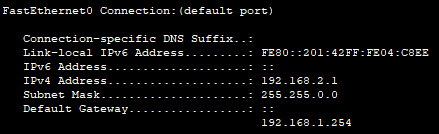
\includegraphics[width=\textwidth,height=\textwidth,keepaspectratio]{./img/test1/user2.png}
        \caption{User 192.168.1.2}
    \end{subfigure}
    ~
    \begin{subfigure}{.45\textwidth}
        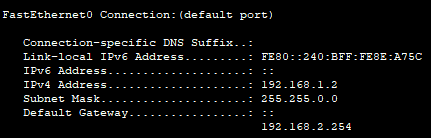
\includegraphics[width=\textwidth,height=\textwidth,keepaspectratio]{./img/test1/admin1.png}
        \caption{Admin 192.168.2.1}
    \end{subfigure}
    \begin{subfigure}{.45\textwidth}
        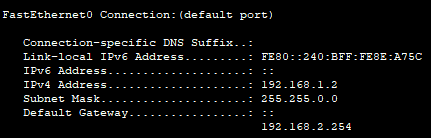
\includegraphics[width=\textwidth,height=\textwidth,keepaspectratio]{./img/test1/admin1.png}
        \caption{Admin 192.168.2.2}
    \end{subfigure}
    \caption{Konfiguration der Systeme}
\end{figure}
\FloatBarrier
\paragraph{Resulate}
Dadurch das die Endsysteme eine /16 Maske haben und das gesamte Netz eigentlich eins ist. Kann man mit dem System, welches am gleichen Switch liegt nicht kommunizieren, aber mit den anderen Endsystemen schon. Dies liegt daran, dass der Router eine /24 Maske hat. Würde der Router auch eine /16 haben, würde auch hier keine Kommunikation zwischen den VLANs zustande kommen.
\begin{figure}[!htb]
    \centering
    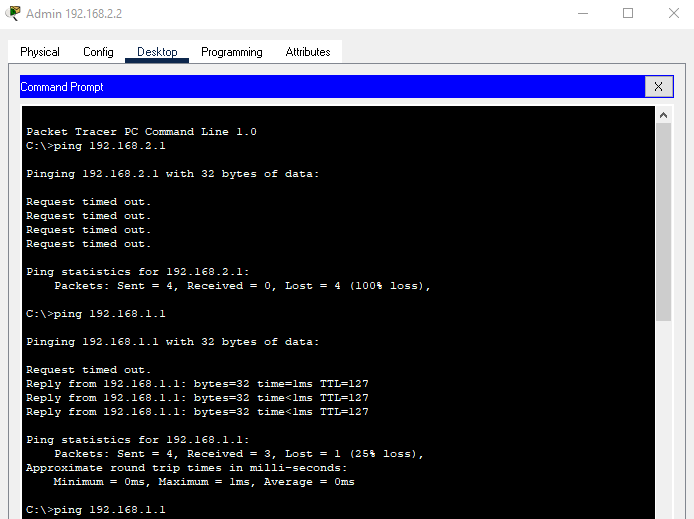
\includegraphics[width=\textwidth,height=.7\textwidth,keepaspectratio]{./img/test1/resultat.png}
    \caption{Admin kann mit User im anderen Netz kommunizieren,aber nicht im gleichen}
\end{figure}
\FloatBarrier

\paragraph{Test für Lösung 2}
\begin{figure}[!htb]
    \centering
    \begin{subfigure}{.45\textwidth}
        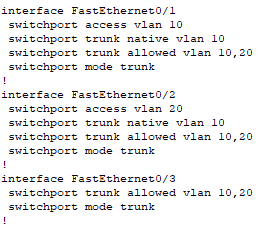
\includegraphics[width=\textwidth,height=\textwidth,keepaspectratio]{./img/test2/S1.png}
        \caption{Switch 1}
    \end{subfigure}
    \begin{subfigure}{.45\textwidth}
        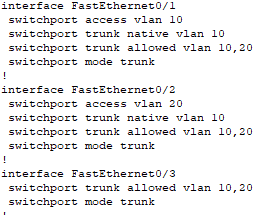
\includegraphics[width=\textwidth,height=\textwidth,keepaspectratio]{./img/test2/S2.png}
        \caption{Switch 2}
    \end{subfigure}
\end{figure}
\FloatBarrier

\paragraph{Resulate}
Wie erwartet können alle Systeme miteinander kommunizieren
\begin{figure}[!htb]
    \centering
    \begin{subfigure}{.8\textwidth}
        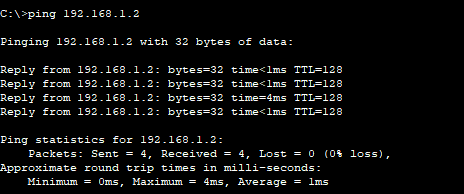
\includegraphics[width=\textwidth,height=\textwidth,keepaspectratio]{./img/test2/User1.png}
    \end{subfigure}
    \begin{subfigure}{.8\textwidth}
        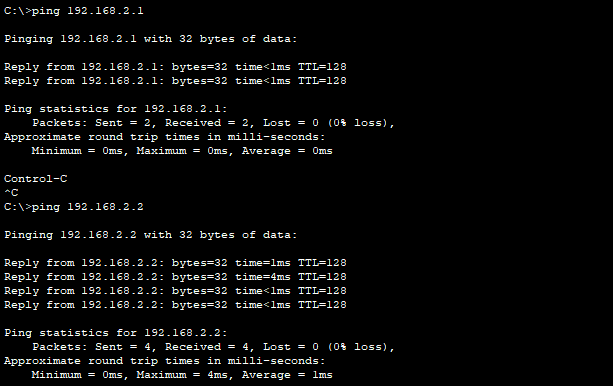
\includegraphics[width=\textwidth,height=\textwidth,keepaspectratio]{./img/test2/user1_t2.png}
    \end{subfigure}
    \caption{192.168.1.1 kommuniziert mit allen Endsystemen}
\end{figure}
\FloatBarrier